\documentclass[11pt,a4paper]{article}
\usepackage[utf8]{inputenc}
\usepackage[T1]{fontenc}
\usepackage{times}
\renewcommand{\ttdefault}{cmtt}
\usepackage{microtype}
\usepackage{amsmath,amssymb}
\usepackage{booktabs}
\usepackage{graphicx}
\usepackage{xcolor}
\usepackage{geometry}
\geometry{margin=25mm}
\usepackage[colorlinks=true,linkcolor=blue!50!black,urlcolor=blue!50!black]{hyperref}

\newcommand{\Dpv}{D_{\mathrm{PV}}}
\newcommand{\Pp}{P_{+}}
\newcommand{\Pm}{P_{-}}
\newcommand{\AL}{\tilde A_{L}}
\newcommand{\Ce}{C_{e}}
\newcommand{\Cpve}{C_{\mathrm{PV},e}}
\newcommand{\Spv}{S_{\mathrm{PV}}}
\newcommand{\dg}{^{\dagger}}

\title{Neff's \texorpdfstring{$\alpha$}{alpha} in the Pauli--Villars multigrid\texorpdfstring{\\}{ }of M\"obius domain-wall fermions: measurements}
\author{Wei-Lun Chen}
\date{October 2026}

\begin{document}
\maketitle

\section{Question}
Neff's form of the domain-wall matrix with $\alpha=0.6$ reduces the iterations of
even-odd CG substantially. In HMC on $24^4$ at $m=0.001$ (setup S below), mixed-precision CG
takes 31996 iterations at $\alpha=0.6$ against 40912 at $\alpha=1$. The multigrid of
RutticeQCD gains little: it takes 362 against 356 in the same runs. On $24^3\times48$ the gain
also depends on the setup (Table~\ref{tab:iter}). We would like to understand where $\alpha$
acts in the multigrid, and whether the coarse space should be built for $D^{(\alpha)}$
instead of $D$.

\section{Operator and multigrid}
Neff's form is $D^{(\alpha)}=DQ$ with $Q$ diagonal in the fifth dimension,
\begin{equation}
Q_0=\Pm+\alpha\Pp,\qquad Q_s=\alpha\ \ (0<s<L_s-1),\qquad Q_{L_s-1}=\Pp+\alpha\Pm .
\end{equation}
$Q$ leaves $\Pm\psi_0$ and $\Pp\psi_{L_s-1}$ unchanged, which make up the quark field, so the
four-dimensional propagator is that of $D$. Up to the overall factor $\alpha$, which a Krylov
method does not see, $\alpha<1$ weights the quark components on the walls by $1/\alpha$
relative to the rest. The outer solver is flexible GCR keeping two directions, on the left
even-odd Pauli--Villars form with $\alpha$ in $D$ only,
\begin{equation}
\AL^{(\alpha)}=(\Cpve^{-1}\Spv)\dg\,Q_e^{-1}\,(\Ce^{-1}S)\,Q_e ,
\end{equation}
with $S$ and $\Spv$ the even-odd Schur complements of $D$ and $\Dpv$ and $\Ce$, $\Cpve$ their
site-diagonal parts on the even sites. The preconditioner is a two-grid cycle
$M=$ Chebyshev smoother, coarse correction $E$, Chebyshev smoother. Its parts are built as
follows:

\begin{center}
\begin{tabular}{@{}ll@{}}
\toprule
part of $M$ & operator it is built from\\
\midrule
test vectors, $P$ (filter and bootstrap) & plain $D$, $\Dpv$\\
coarse operators $P\dg DP$, $P\dg\Dpv\dg P$ & plain $D$, $\Dpv$\\
site-local factors $O_R=1$, $O_M=\Ce Q_e\Cpve\dg$, $O_L=Q_e^{-1}$ of $E$ & $\AL^{(\alpha)}$\\
Chebyshev smoother and the top $\lambda_{\rm hi}$ of its interval & $\AL^{(\alpha)}$\\
\bottomrule
\end{tabular}
\end{center}

\noindent The correction follows from
$\AL^{(\alpha)\,-1}=Q_e^{-1}S^{-1}\Ce Q_e\Cpve\dg(\Spv\dg)^{-1}$:
\begin{equation}
E=O_L\,\pi P(P\dg DP)^{-1}P\dg\iota\;O_M\;\pi P(P\dg\Dpv\dg P)^{-1}P\dg\iota\;O_R ,
\end{equation}
with $\iota$ and $\pi$ the embedding of the even sites and the projection onto them. Every $\alpha$ therefore shares one
setup. For the right form the correction is exact on the vectors $P$ is built from; for the
left form it is not, already at $\alpha=1$.

\paragraph{Setups.} M\"obius $(b,c)=(1.5,0.5)$, $L_s=8$, $m_{\rm PV}=1$, $\alpha_{\rm PV}=1$.
Setup S: $M_5=1.0$, stout links ($\rho=0.1$, 3 steps), Chebyshev with 8 steps on
$[\lambda_{\rm hi}/10,\lambda_{\rm hi}]$. Setup B: $M_5=1.8$, unsmeared links, 12 steps on
$[\lambda_{\rm hi}/30,\lambda_{\rm hi}]$. Aggregates of $4^4$ sites with the whole fifth
dimension, 32 test vectors (16 filtered low modes, each lifted to two columns), coarse solves
in single precision to $|r|^2/|b|^2<10^{-2}$, GCR(2) to $10^{-18}$. Configurations: quenched,
plaquette action at $\beta=6.0$. The $12^4$ one has one unpaired near-zero mode ($Q=+1$).
All runs on one GPU.

\section{Iterations}
\begin{table}[h]
\centering
\caption{GCR(2) iterations with the multigrid, $\alpha=0.6$ / $\alpha=1$.}
\label{tab:iter}
\begin{tabular}{@{}lcccc@{}}
\toprule
 & \multicolumn{2}{c}{$12^4$} & \multicolumn{2}{c}{$24^3\times48$}\\
$m$ & S & B & S & B\\
\midrule
$0.1$   & $8/9$   & $7/9$   & $13/16$ & $7/9$\\
$0.01$  & --      & --      & $15/15$ & $15/17$\\
$0.001$ & $14/13$ & $14/15$ & $28/27$ & $26/28$\\
\bottomrule
\end{tabular}
\end{table}
In setup B, $\alpha=0.6$ saves one to three iterations at every mass on both volumes. In
setup S it saves at $m=0.1$ and loses one at $m=0.001$. The $12^4$ lattice shows the same
pattern as $24^3\times48$, so the measurements below are on $12^4$.

\section{Residual histories}
\begin{figure}[h]
\centering
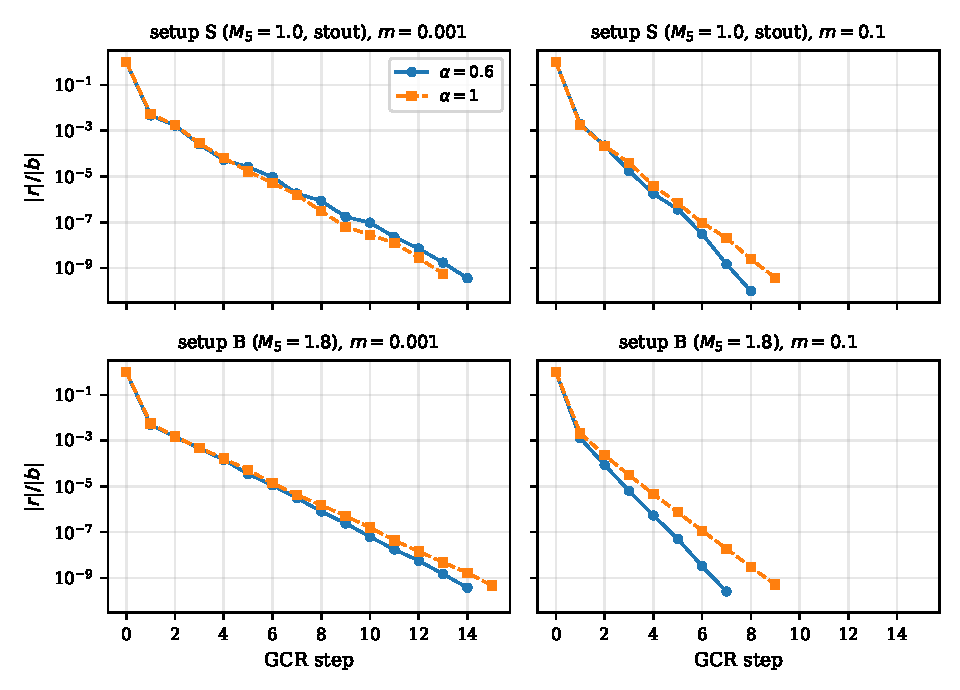
\includegraphics[width=0.85\textwidth]{fig_history_12.pdf}
\caption{GCR(2) residual histories on $12^4$, one random right-hand side.}
\label{fig:hist}
\end{figure}
\begin{table}[h]
\centering
\caption{Mean reduction of $|r|/|b|$ per GCR step, $\alpha=0.6$ / $\alpha=1$, over steps
1--4 and from step 4 to convergence. The first step reduces $|r|/|b|$ to $1$--$6\times10^{-3}$
in every case.}
\label{tab:rate}
\begin{tabular}{@{}llcc@{}}
\toprule
setup & $m$ & steps 1--4 & step 4 to end\\
\midrule
S & $0.001$ & $0.224/0.228$ & $0.304/0.274$\\
S & $0.1$   & $0.097/0.130$ & $0.086/0.157$\\
B & $0.001$ & $0.310/0.306$ & $0.276/0.313$\\
B & $0.1$   & $0.075/0.130$ & $0.078/0.162$\\
\bottomrule
\end{tabular}
\end{table}
The difference comes from the rate after the first cycle (Fig.~\ref{fig:hist},
Table~\ref{tab:rate}). At $m=0.1$, $\alpha=0.6$ converges faster from the second step on, by
a factor of two per step in setup B. At $m=0.001$ the first four steps agree within a few
percent in both setups. Setup S at $m=0.001$ then slows down with $\alpha=0.6$, with several
steps that reduce the residual by only $0.36$--$0.56$, once $|r|/|b|$ is below about
$10^{-4}$.

\section{Spectra}
\paragraph{\texorpdfstring{$\AL^{(\alpha)}$}{A_L} without the multigrid.} Implicitly restarted Arnoldi, 48
eigenvalues of smallest real part and 4 of largest magnitude:
\begin{center}
\begin{tabular}{@{}llccc@{}}
\toprule
setup & $m$ & $|\lambda_0|$, $\alpha=0.6/1$ & $|\lambda_{47}|$ & $|\lambda|_{\max}$\\
\midrule
S & $0.001$ & $3.72/2.32\times10^{-4}$ & $0.155/0.096$ & $1.981/1.980$\\
S & $0.1$   & $3.63/2.29\times10^{-2}$ & $0.151/0.099$ & $1.981/1.980$\\
B & $0.001$ & $1.49/1.05\times10^{-3}$ & $0.118/0.082$ & $4.442/4.454$\\
B & $0.1$   & $4.10/3.04\times10^{-2}$ & $0.074/0.082$ & $4.442/4.453$\\
\bottomrule
\end{tabular}
\end{center}
$\alpha=0.6$ raises the smallest eigenvalue by a factor $1.35$--$1.6$ and leaves the largest
unchanged to $0.3\%$. The factor is $1.6$ in S at both masses and $1.42$, $1.35$ in B.

\paragraph{\texorpdfstring{$\AL^{(\alpha)}M$}{A_L M}.} The same Arnoldi on the preconditioned operator, with $M$ built
as in the solver but with exact coarse solves (double precision, $10^{-20}$), so that $M$ is
linear. $\kappa$ is the condition number $1/|y\dg x|$ of $\lambda_0$, from the left and right
eigenvectors; $\|I-\AL S\|_2$ and $\|I-\AL E\|_2$ are those of the smoother and of the
correction alone.
\begin{center}
\begin{tabular}{@{}llcccccc@{}}
\toprule
setup & $m$ & $\alpha$ & ${\rm Re}\,\lambda_0$ & $\kappa(\lambda_0)$ & $|\lambda|_{\max}$ & $\|I-\AL S\|_2$ & $\|I-\AL E\|_2$\\
\midrule
S & $0.001$ & $0.6$ & $0.499$ & $17.8$ & $4.27$ & $1.038$ & $2.83\times10^4$\\
  &         & $1$   & $0.863$ & $8.1$  & $5.48$ & $1.022$ & $1.90\times10^4$\\
S & $0.1$   & $0.6$ & $0.865$ & $8.5$  & $8.08$ & $0.674$ & $3.29\times10^4$\\
  &         & $1$   & $0.902$ & $8.0$  & $6.09$ & $0.776$ & $2.22\times10^4$\\
B & $0.001$ & $0.6$ & $0.687$ & $9.2$  & $1.71$ & $1.173$ & $3.87\times10^3$\\
  &         & $1$   & $0.830$ & $15.3$ & $1.75$ & $1.117$ & $2.81\times10^3$\\
B & $0.1$   & $0.6$ & $0.952$ & $11.6$ & $1.30$ & $0.677$ & $1.22\times10^3$\\
  &         & $1$   & $0.913$ & $6.1$  & $1.28$ & $0.779$ & $9.13\times10^2$\\
\bottomrule
\end{tabular}
\end{center}
The spread $|\lambda|_{\max}/{\rm Re}\,\lambda_0$ is larger with $\alpha=0.6$ in three cases and
unchanged in B at $m=0.1$, where $\alpha=0.6$ gains the most. The eigenvalues of this linear
$\AL^{(\alpha)}M$ therefore do not follow the convergence rates of Table~\ref{tab:rate}. At
$m=0.1$, $\alpha=0.6$ reduces $\|I-\AL S\|_2$ by $13\%$ in both setups. With $\alpha=0.6$,
$\|I-\AL E\|_2$ is larger by a factor $1.34$--$1.49$ in all four cases.

\section{The cycle on the low modes of \texorpdfstring{$\AL^{(\alpha)}$}{A_L}}
For the 8 eigenvectors $x$ of $\AL^{(\alpha)}$ of smallest real part ($|x|=1$, eigenpair
residuals below $4\times10^{-8}$) we measure
\begin{equation}
\delta_X(x)=\min_c|x-c\,\AL^{(\alpha)}Xx| ,\qquad X=E,\ M,
\end{equation}
the part of $\AL^{(\alpha)}Xx$ off the direction of $x$. GCR chooses the scale $c$ itself, so
$\delta_X$ is the quantity that matters for one step: $\delta=0$ when $X$ inverts
$\AL^{(\alpha)}$ on $x$, $\delta=1$ when $\AL^{(\alpha)}Xx\perp x$.
\begin{table}[h]
\centering
\caption{$\delta_M$ over the 8 lowest eigenvectors, median (largest), with exact coarse
solves and with the solver's $10^{-2}$.}
\label{tab:defect}
\begin{tabular}{@{}llcccc@{}}
\toprule
 & & \multicolumn{2}{c}{exact} & \multicolumn{2}{c}{$10^{-2}$}\\
setup & $m$ & $\alpha=0.6$ & $\alpha=1$ & $\alpha=0.6$ & $\alpha=1$\\
\midrule
S & $0.001$ & $0.917\ (0.994)$ & $0.620\ (0.977)$ & $0.990\ (0.995)$ & $0.958\ (0.979)$\\
S & $0.1$   & $0.918\ (0.977)$ & $0.737\ (0.882)$ & $0.972\ (0.993)$ & $0.889\ (0.966)$\\
B & $0.001$ & $0.788\ (0.919)$ & $0.668\ (0.887)$ & $0.828\ (0.919)$ & $0.689\ (0.887)$\\
B & $0.1$   & $0.339\ (0.398)$ & $0.340\ (0.407)$ & $0.366\ (0.454)$ & $0.364\ (0.449)$\\
\bottomrule
\end{tabular}
\end{table}
With $\alpha=0.6$ the cycle treats the low modes worse in three of the four cases, by
$0.30$, $0.18$ and $0.12$ in the median with exact solves (S at $m=0.001$ and $0.1$, B at
$m=0.001$), and the same in B at $m=0.1$. The loss is larger in setup S. The correction
alone gives $\delta_E=0.98$--$1.00$ in every case, at $\alpha=1$ too: on these eigenvectors
$\AL^{(\alpha)}Ex$ is nearly orthogonal to $x$. The reduction of these modes in one cycle,
where there is any, comes from the full cycle.

\section{A reading}
The data are consistent with two effects of $\alpha$ of opposite sign. This reading is a
hypothesis; the two effects have not been separated in a solve.
\begin{enumerate}
\item The smoother works on $\AL^{(\alpha)}$, and on the part of the spectrum it covers
$\alpha=0.6$ helps it ($\|I-\AL S\|_2$ lower by $13\%$ at $m=0.1$).
\item $P$ and the coarse operators are those of $D$, and with $\alpha=0.6$ the cycle treats
the low modes of $\AL^{(\alpha)}$ worse (Table~\ref{tab:defect}).
\end{enumerate}
At $m=0.1$ the low modes do not set the cost, and the first effect gives the faster rate in
both setups. At $m=0.001$ the low modes matter. In B the smoother interval is wide and the
loss on the low modes is small, so the net effect is still a gain. In S the interval is
narrow, the coarse correction carries the low modes, the loss is largest, and $\alpha$ costs
an iteration. The late slowdown of S at $m=0.001$ in Fig.~\ref{fig:hist}, after the
residual has fallen below $10^{-4}$, fits a remainder made of low modes.

\section{Questions}
\begin{enumerate}
\item Should the coarse space be built from the near-null vectors of $D^{(\alpha)}$, which are
$Q^{-1}$ times those of $D$, when the outer operator carries $\alpha$? Our aggregates keep
the whole fifth dimension and split it only by $\Gamma_5$ chirality, so we expect $Q^{-1}y$
to lie outside the range of $P$ in general; we have not checked this. A $P$ built from
$Q^{-1}y$ has not been tried.
\item Is $\delta_E\approx1$ on the low eigenvectors expected for the left form, with only the
smoothed cycle reducing them?
\item For comparison, an earlier Bridge++ implementation uses the same $D^{(\alpha)}=DQ$, in
the whole-lattice operator $(\Dpv C_{\rm PV}^{-1})\dg C^{-1}D$ with $C$ the site-local block,
and forms the coarse operator from the operator with $\alpha$. On a $12^4$ cold configuration
at $\beta=5.7$ and $m=0.005$, $\alpha=0.6$ raised $\lambda_{\max}$ there from $4.66$ to $10.6$,
and its multigrid took 266 iterations against 210 at $\alpha=1$. Here $\lambda_{\max}$ of
$\AL^{(\alpha)}$ does not change with $\alpha$. Would one expect the difference from the
whole-lattice form against the even-odd left form, from the coarse space, or from the
configuration? One candidate for the form: $\AL^{(\alpha)}$ is similar to
$S_{\rm PV}\dg C_{\rm PV}^{\dagger\,-1}Q_e^{-1}C_e^{-1}S$, with the site-local factors between
the two Schur complements, while in the whole-lattice operator $Q^{-1}$ multiplies $C^{-1}D$
from one side only.
\item With $\alpha$ in $D_{\rm PV}$ as well (the code of 2026-10-11, $12^4$, the same setup and
coarse factors), the multigrid took 25 GCR(2) cycles at $\alpha=0.6$ (three right-hand sides)
and 58 at $\alpha=0.5$ (one right-hand side); FGMRES(16) took 45--46 at $\alpha=0.5$. With
$\alpha$ in $D$ only it took 24 at $\alpha=0.5$. What makes the cycle fail there?
\end{enumerate}

\paragraph{Data.} The tables and the figure script are in \texttt{docs/alpha\_study/}.

\end{document}
